\documentclass{beamer}
\usetheme{Madrid}
\usefonttheme{structurebold}

\AtBeginSection[]{
  \begin{frame}
  \vfill
  \centering
  \begin{beamercolorbox}[sep=8pt,center,shadow=true,rounded=true]{title}
    \usebeamerfont{title}\insertsectionhead\par%
  \end{beamercolorbox}
  \vfill
  \end{frame}
}

\usepackage{lmodern}
\usepackage{fontawesome}
\usepackage{pgf}
\usepackage{tikz}
\usetikzlibrary{arrows,automata}
\usetikzlibrary{positioning}
\usetikzlibrary{matrix,positioning,tikzmark}
\usepackage{pict2e}
\usepackage{multirow}

\tikzset{
    font={\fontsize{8pt}{8}\selectfont},
    state/.style={
           rectangle,
           rounded corners,
           draw=black, very thick,
           minimum height=1.3em,
           inner sep=2pt,
           text centered,
           },
    invisible/.style={opacity=0},
    visible on/.style={alt={#1{}{invisible}}}, alt/.code args={<#1>#2#3}{%
    \alt<#1>{\pgfkeysalso{#2}}{\pgfkeysalso{#3}} % \pgfkeysalso doesn't change the path
    },
}

%\useoutertheme[footline=authortitle]{miniframes}

\title{Semantics Driven Agent Programming}
\author[Francesco Antoniazzi]{\textit{Candidato}: Ing. Francesco Antoniazzi \\
\textit{Relatore}: Prof. Tullio Salmon Cinotti \\
\textit{Coordinatore Dottorato}: Prof. Davide Sangiorgi}
\centering
\date{Lyon - Bologna, 2 Aprile 2020\\\vspace{5mm} \footnotesize{\texttt{francesco.antoniazzi}\faAt \texttt{unibo.it}}}
\institute{Dottorato in Computer Science and Engineering - XXXII ciclo \\ Alma Mater Studiorum Università di Bologna}

\makeatletter
\setbeamertemplate{footline}
{
  \leavevmode%
  \hbox{%
  \begin{beamercolorbox}[wd=.333333\paperwidth,ht=2.25ex,dp=1ex,center]{author in head/foot}%
    \usebeamerfont{author in head/foot}\insertshortauthor%~~\beamer@ifempty{\insertshortinstitute}{}{(\insertshortinstitute)}
  \end{beamercolorbox}%
  \begin{beamercolorbox}[wd=.555555\paperwidth,ht=2.25ex,dp=1ex,center]{title in head/foot}%
    \usebeamerfont{title in head/foot}\insertshorttitle
  \end{beamercolorbox}%
  \begin{beamercolorbox}[wd=.111111\paperwidth,ht=2.25ex,dp=1ex,right]{date in head/foot}%
%    \usebeamerfont{date in head/foot}\insertshortdate{}\hspace*{2em}
    \insertframenumber{} / \inserttotalframenumber\hspace*{2ex} 
  \end{beamercolorbox}
}%
  \vskip0pt%
}
\makeatother

\begin{document}
\maketitle

\begin{frame}{Outline}
\tableofcontents
\end{frame}

\section{Internet of Things}
\subsection{Breaking Fragmentation}
\begin{frame}{State of the Art}
\begin{itemize}
    \item Providing internet connectivity to all sort of devices: everyday items, machines, clothing, buildings, ...,  in order to collect information on entities and environments. And realize applications;
    \item Interoperability issues: vertical silos;
    \item Breaking fragmentation means creating a bridge at some level of ISO-OSI stack;
\end{itemize}
\end{frame}

\begin{frame}{Breaking fragmentation}
\includegraphics[width=.8\textwidth]{OSILayers.png}
\end{frame}

\begin{frame}{Breaking fragmentation}
\begin{flushleft}
Let us just consider Application layer protocols, like MQTT and AMQP. 

The \textit{topic} communication implies that there is an agreement on the semantics among application:
\begin{enumerate}
    \item<1-> The topic URI is interpreted in the same way; \\
    \textit{this is the place in which temperature information should be stored}
    \item<2-> The exchanged information has the same format; \\
    \textit{information should be provided as a JSON file compliant with a specific JSONSchema}
    \item<3-> The exchanged information has the same semantics; \\
    \textit{no misunderstanding is possible on the meaning of the received value: }\textcolor{blue}{\texttt{mouse}} \textit{means `~\includegraphics[scale=.015]{mouse}' for all participants, and is never intended as `~\faMousePointer'}
\end{enumerate}
\end{flushleft}
\end{frame}

\begin{frame}{Breaking fragmentation}
But how do we agree on all this, if applications are developed 
in different places, different times, by different people, with different purposes?

\includegraphics[scale=.05]{rdf.png}

The Resource Description Framework (RDF) can enrich with semantics all the Application and Information level of the IoT.
\end{frame}

\section{Semantic Internet of Things}
\begin{frame}{What's a \textit{Thing}?}
\begin{block}{IEEE definition}
\textit{The Thing is any physical object \textbf{relevant} from a user or application perspective.}
\end{block} \pause
\begin{block}{W3C definition}
\textit{Things can be \textbf{virtual representations} of physical or abstract entities. They can be connected or not connected. Each thing can have one or more virtual representations. Things can have histories, and have identities, rich \textbf{descriptions}, services, access control and data handling policies. They have URIs.}
\end{block}
\vfill
\footnotesize{Ref. \cite{liu2016comparison}}
\end{frame}

\subsection{IEEE approach}
\begin{frame}{Internet of Musical Things (IoMusT) Ontology}
\framesubtitle{IEEE approach}
\begin{flushleft}
The Internet of Musical Things is the ensemble of interfaces, protocols and representations of music-related information that enable services and applications serving a musical purpose based on interactions between humans and Musical Things or between Musical Things themselves, in physical and/or digital realms.\\
\vspace{1mm}
Music-related information refers to data sensed and processed by a Musical Thing, and/or exchanged with a human or with another Musical Thing \cite{turchet2018IoMusT}.
\end{flushleft}
\end{frame}

\subsection{IoMusT Ontology}
\begin{frame}{Internet of Musical Things (IoMusT) Ontology}
\framesubtitle{IEEE approach}
\includegraphics[scale=.5]{onto_schema.png}
\begin{itemize}
    \item Is IoMusT a subcase of IoT? 
    \item It presents an approach, a model to realize a semantic and fully interoperable IoT connecting different fields incrementally;
    \item Topic completely unexplored in literature: music+IoT+semantics \cite{turchet2020internet};
\end{itemize}
\end{frame}

\begin{frame}{IoMusT Ontology}
\begin{scriptsize}
\begin{table}
    \begin{tabular}{r|c|c|c|c|c|c|c|c|c|}
     & \rotatebox{90}{\texttt{ns:Bob}} & \rotatebox{90}{\texttt{ns:Wardrobe}} & \rotatebox{90}{\texttt{ns:SmartCar}} & \rotatebox{90}{\texttt{ns:Violin}} & \rotatebox{90}{\texttt{ns:SmartViolin}} & \rotatebox{90}{\texttt{ns:TShirt}} & \rotatebox{90}{\texttt{ns:StageLight}} & \rotatebox{90}{\texttt{ns:VR\_HeadSet}} &
     \rotatebox{90}{\begin{tabular}{@{}c@{}}\texttt{ns:HeartBeatSensor} \\ for music experiment \end{tabular}} \\
     \hline
    \texttt{foaf:Person} & \faCheck  &  &  &  &  &  &  &  &\\ \hline
    \texttt{iot:Thing} &  &  \faCheck &  \faCheck & \faCheck  & \faCheck & \faCheck  & \faCheck  & \faCheck & \faCheck \\ \hline
    \texttt{iot:SmartThing} &  &  &  \faCheck &  &  \faCheck &  & \faCheck & \faCheck & \\ \hline
    \texttt{iot:ConnectedThing} &  &  &  &  &  \faCheck &  & \faCheck & \faCheck & \faCheck \\ \hline
    \texttt{iot:WearableThing} &  &  &  &  & & \faCheck &  &  \faCheck & \faCheck \\ \hline
    \texttt{mo:Instrument} &  &   &  & \faCheck &  \faCheck &  &  &  & \\ \hline
    \texttt{iomust:MusicalThing} &  &   &  & \faCheck  &  \faCheck &  &  \faCheck &  & \faCheck \\ \hline
    \texttt{iomust:SmartMusicalThing} & &  &   &  &  \faCheck &  & \faCheck  &  & \\ \hline
    \texttt{iomust:SmartInstrument} &  &  &  &  &  \faCheck &  &  &  & \\ \hline
    \texttt{iomust:StageEquipment} item &  &  &  &  &  &  & \faCheck &  &  \\ \hline
    \texttt{iomust:WearableMusicalThing} &  &  &  &  &  &  &  &  & \faCheck\\ \hline
    \end{tabular}
\end{table}
\end{scriptsize}
\end{frame}

\begin{frame}{IoMusT Ontology}
\begin{footnotesize}
\begin{block}{Rule Example 1 (not reversible!)}
\begin{multline*}
\texttt{?s a iot:Thing, mo:Instrument} 
\Rightarrow
\texttt{?s a iomust:MusicalThing}
\end{multline*}
Where the Musical Thing is \textit{a thing used to produce or enjoy music, with reference to its context}.

\end{block}\pause
\begin{block}{Rule Example 2}
\begin{multline*}
\texttt{?e co:elementOf ?s; a iomust:MusicalThing. ?s a co:collection } \\
\Leftrightarrow
\texttt{?s a iomust:StageEquipment}
\end{multline*}

\end{block} 
\end{footnotesize}
\end{frame}

\begin{frame}{IoMusT Ontology example I}
\begin{flushleft}
How do we describe a Smart Guitar with:
\begin{enumerate}
    \item An IMU sensor unit;
    \item A contact microphone;
    \item A loudspeaker;
\end{enumerate}
\end{flushleft}
\end{frame}

\begin{frame}{IoMusT Ontology example I}
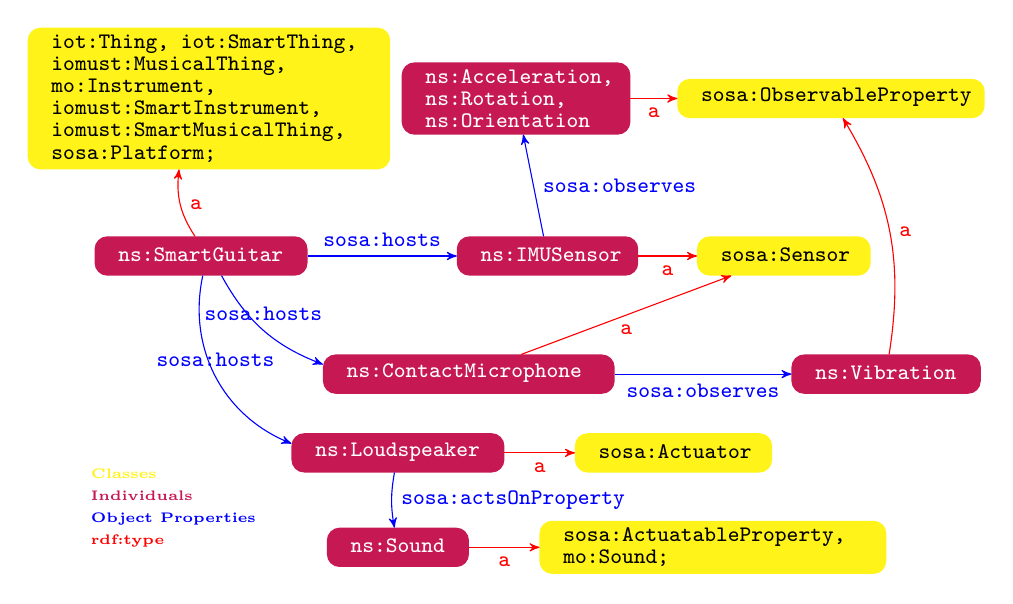
\begin{tikzpicture}[->,>=stealth']

\node[state,draw=purple!90,fill=purple!90,text=white,align=center] (SMARTGUITAR) {
\begin{tabular}{l}
  \parbox{2cm}{\texttt{ns:SmartGuitar}}
   \end{tabular}
};

\node[state,draw=none,yshift=-3.2cm,align=center, node distance=-1cm] (LEGEND) {
\begin{tabular}{l}
  \parbox{2.7cm}{
  \textbf{\tiny{\textcolor{yellow!90}{Classes}\\\textcolor{purple!90}{Individuals}\\\textcolor{blue}{Object Properties}\\\textcolor{red}{rdf:type}}}}
  \end{tabular}
};
  
 % State: ACK with different content
 \node[state,  yshift=2cm, right of=SMARTGUITAR, node distance=0.1cm, anchor=center, draw=yellow!90,fill=yellow!90,align=center] (SGTYPES) {%
    \begin{tabular}{l} 
        \parbox{3.9cm}{\texttt{iot:Thing, iot:SmartThing,\\iomust:MusicalThing, mo:Instrument,\\iomust:SmartInstrument,\\iomust:SmartMusicalThing, sosa:Platform;}}
    \end{tabular}
};
  
   % State: ACK with different content
\node[state, yshift=0cm, right of=SMARTGUITAR, node distance=4.4cm, anchor=center, draw=purple!90,fill=purple!90,align=center,text=white] (IMUSENSOR) {%
    \begin{tabular}{l}
        \parbox{1.6cm}{\texttt{ns:IMUSensor}}
    \end{tabular}
};
  
\node[state, yshift=-1.5cm, right of=SMARTGUITAR, node distance=3.4cm, anchor=center, draw=purple!90,fill=purple!90,align=center,text=white] (CONTACTMIC) {%
    \begin{tabular}{l} 
        \parbox{3cm}{\texttt{ns:ContactMicrophone}}
    \end{tabular}
};
  
\node[state, yshift=-2.5cm, right of=SMARTGUITAR, node distance=2.5cm, anchor=center, draw=purple!90,fill=purple!90,align=center,text=white] (LOUDSPEAKER) {%
    \begin{tabular}{l} 
        \parbox{2cm}{\texttt{ns:Loudspeaker}}
    \end{tabular}
};
  
\node[state, yshift=0cm, right of=IMUSENSOR, node distance=3cm, anchor=center, draw=yellow!90,fill=yellow!90,align=center] (SENSORS) {%
    \begin{tabular}{l}
        \parbox{1.5cm}{\texttt{sosa:Sensor}}
    \end{tabular}
};
  
\node[state, yshift=0cm, right of=LOUDSPEAKER, node distance=3.5cm, anchor=center, draw=yellow!90,fill=yellow!90,align=center] (ACTUATORS) {%
    \begin{tabular}{l}
        \parbox{1.8cm}{\texttt{sosa:Actuator}}
    \end{tabular}
};
  
\node[state, yshift=0cm, right of=SGTYPES, node distance=3.9cm, anchor=center, draw=purple!90,fill=purple!90,align=center,text=white] (IMUHOSTS) {%
    \begin{tabular}{l} 
        \parbox{2.2cm}{\texttt{ns:Acceleration,\\ns:Rotation,\\ns:Orientation}}
    \end{tabular}
};
  
\node[state, yshift=0cm,  right of=IMUHOSTS, node distance=4cm, anchor=center, draw=yellow!90,fill=yellow!90,align=center] (OBSERVABLEPROPERTY) {%
    \begin{tabular}{l} 
        \parbox{3.2cm}{\texttt{sosa:ObservableProperty}}
    \end{tabular}
};
  
\node[state, yshift=0cm, right of=CONTACTMIC, node distance=5.3cm, anchor=center, draw=purple!90,fill=purple!90,align=center,text=white] (VIBRATION) {%
    \begin{tabular}{l}
        \parbox{1.7cm}{\texttt{ns:Vibration}}
    \end{tabular}
};
  
\node[state, yshift=-1.2cm,  right of=LOUDSPEAKER, node distance=0cm, anchor=center, draw=purple!90,fill=purple!90,align=center,text=white] (SOUND)  {%
    \begin{tabular}{l} 
        \parbox{1.1cm}{\texttt{ns:Sound}}
    \end{tabular}
};
  
\node[state, yshift=0cm, right of=SOUND, node distance=4cm, anchor=center, draw=yellow!90,fill=yellow!90,align=center] (ACTUATABLEPROPERTY) {%
    \begin{tabular}{l}
        \parbox{3.7cm}{\texttt{sosa:ActuatableProperty, mo:Sound;}}
    \end{tabular}
};
 
\path (SMARTGUITAR)     edge[bend left=20,draw=red]  node[anchor=west]{\textcolor{red}{\texttt{a}}}   (SGTYPES)
(SMARTGUITAR)   edge[anchor=south,draw=blue] node[]{\textcolor{blue}{\texttt{sosa:hosts}}}                      (IMUSENSOR)  
(SMARTGUITAR)   edge[bend right=40,draw=blue] node[anchor=south, above]{\textcolor{blue}{\texttt{sosa:hosts}}}  (LOUDSPEAKER)  
(SMARTGUITAR)   edge[bend right=20,draw=blue] node[anchor=south, above]{\textcolor{blue}{\texttt{sosa:hosts}}}  (CONTACTMIC)
(IMUSENSOR)     edge[draw=red] node[anchor=north]{\textcolor{red}{\texttt{a}}}                                (SENSORS)
(LOUDSPEAKER)   edge[draw=red] node[anchor=north]{\textcolor{red}{\texttt{a}}}                                (ACTUATORS)
(CONTACTMIC)    edge[draw=red] node[anchor=north]{\textcolor{red}{\texttt{a}}}                                (SENSORS)
(IMUSENSOR)     edge[draw=blue] node[anchor=west]{\textcolor{blue}{\texttt{sosa:observes}}}       (IMUHOSTS)
(IMUHOSTS)     	edge[draw=red] node[anchor=north]{\textcolor{red}{\texttt{a}}}                                (OBSERVABLEPROPERTY)
(CONTACTMIC)    edge[draw=blue] node[anchor=north]{\textcolor{blue}{\texttt{sosa:observes}}}                    (VIBRATION)
(VIBRATION)     edge[bend right=20, draw=red] node[anchor=west]{\textcolor{red}{\texttt{a}}}                                (OBSERVABLEPROPERTY)
(LOUDSPEAKER)   edge[bend right=10, draw=blue] node[anchor=west]{\textcolor{blue}{\texttt{sosa:actsOnProperty~~~~}}}         (SOUND)
(SOUND)     	edge[draw=red] node[anchor=north]{\textcolor{red}{\texttt{a}}}                                (ACTUATABLEPROPERTY);   

\end{tikzpicture}
\end{frame}

\begin{frame}{IoMusT Ontology example II}
\begin{flushleft}
How do we describe an IoMusT application:
\begin{enumerate}
    \item A music performance made by someone;
    \item Using a Smart guitar belonging to someone;
    \item Starting at a specific time;
    \item Having a specific duration;
\end{enumerate}
\end{flushleft}
\end{frame}

\begin{frame}{IoMusT Ontology example II}
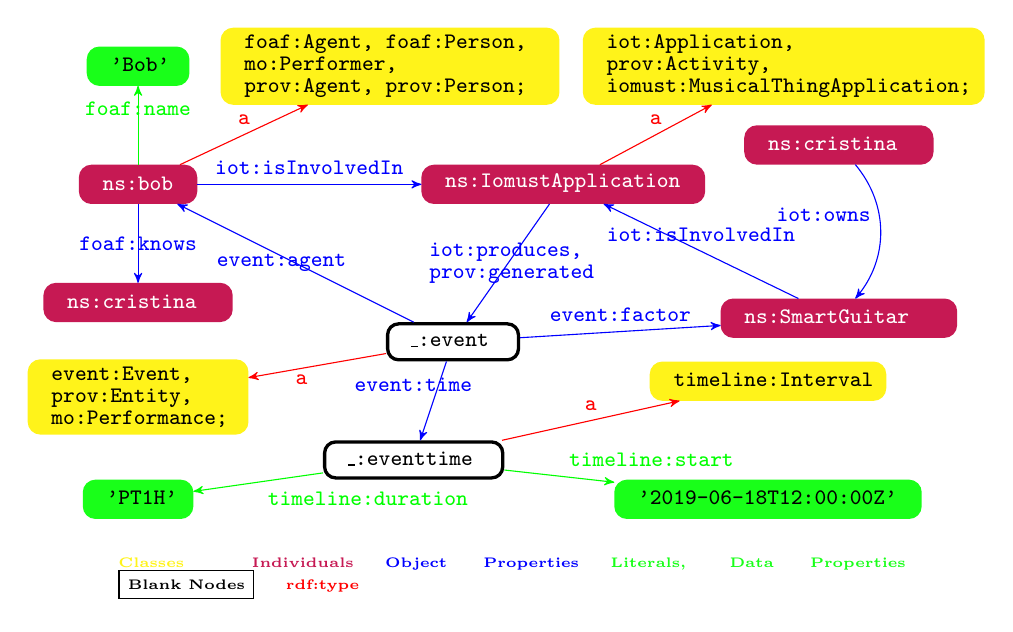
\begin{tikzpicture}[->,>=stealth']

\node[state,draw=purple!90,fill=purple!90,text=white,align=center] (BOB) {
\begin{tabular}{l}
  \parbox{0.8cm}{\texttt{ns:bob}}
   \end{tabular}
};
  
 % State: ACK with different content
 \node[state,  yshift=1.5cm, right of=BOB, node distance=3.2cm, anchor=center, draw=yellow!90,fill=yellow!90,align=center] (BOBTYPES) {%
    \begin{tabular}{l} 
        \parbox{3.6cm}{\texttt{foaf:Agent, foaf:Person, 
                mo:Performer,\\prov:Agent, prov:Person;}}
    \end{tabular}
};

 % State: ACK with different content
 \node[state,  yshift=1.5cm, node distance=0cm, anchor=center, draw=green!90,fill=green!90,align=center] (BOBNAME) {%
    \begin{tabular}{l} 
        \parbox{0.6cm}{\texttt{'Bob'}}
    \end{tabular}
};
  
   % State: ACK with different content
\node[state, yshift=-1.5cm, anchor=center, draw=purple!90,fill=purple!90,align=center,text=white] (CRISTINA) {%
    \begin{tabular}{l}
        \parbox{1.7cm}{\texttt{ns:cristina}}
    \end{tabular}
};
  
\node[state, right of=BOB, node distance=5.4cm, anchor=center, draw=purple!90,fill=purple!90,align=center,text=white] (APPLICATION) {%
    \begin{tabular}{l} 
        \parbox{2.9cm}{\texttt{ns:IomustApplication}}
    \end{tabular}
};

\node[state, anchor=center, 
right of=APPLICATION, 
draw=purple!90,fill=purple!90,
align=center,text=white, yshift=0.5cm, node distance=3.5cm] (CRISTINATWO) {%
    \begin{tabular}{l}
        \parbox{1.7cm}{\texttt{ns:cristina}}
    \end{tabular}
};

 \node[state, right of=BOBTYPES, node distance=5cm, anchor=center, draw=yellow!90,fill=yellow!90,align=center] (APPLICATIONTYPES) {%
    \begin{tabular}{l} 
        \parbox{4.4cm}{\texttt{iot:Application, prov:Activity,\\
        iomust:MusicalThingApplication;}}
    \end{tabular}
};

\node[state,yshift=-1.7cm,draw=purple!90,right of=APPLICATION, node distance=3.5cm, fill=purple!90,text=white,align=center] (SMARTGUITAR) {
\begin{tabular}{l}
  \parbox{2.3cm}{\texttt{ns:SmartGuitar}}
   \end{tabular}
};

\node[state, 
%draw=purple!90,
right of=CRISTINA, node distance=4cm, yshift=-.5cm,
%fill=purple!90,
%text=white,
align=center] (EVENT) {
\begin{tabular}{l}
  \parbox{1cm}{\texttt{\_:event}}
   \end{tabular}
};

 \node[state, yshift=-0.7cm, right of=EVENT, node distance=-4cm, anchor=center, draw=yellow!90,fill=yellow!90,align=center] (EVENTTYPES) {%
    \begin{tabular}{l} 
        \parbox{2.1cm}{\texttt{event:Event, prov:Entity, mo:Performance;}}
    \end{tabular}
};

\node[state,draw=none,right of=CRISTINA, node distance=4.8cm, yshift=-3.5cm,align=center] (LEGEND) {
\begin{tabular}{l}
  \parbox{10cm}{
  \textbf{\tiny{\textcolor{yellow!90}{Classes} \hspace{.4cm}\textcolor{purple!90}{Individuals}\hspace{.4cm}\textcolor{blue}{Object Properties}\hspace{.4cm}\textcolor{green!90}{Literals, Data Properties}\hspace{.4cm}\framebox{Blank Nodes}\hspace{.4cm}\textcolor{red}{rdf:type}}}}
  \end{tabular}
};

\node[state,yshift=-2cm, 
%draw=purple!90,
right of=CRISTINA, node distance=3.5cm,
%fill=purple!90,
%text=white,
align=center] (EVENTTIME) {
\begin{tabular}{l}
  \parbox{1.6cm}{\texttt{\_:eventtime}}
   \end{tabular}
};

\node[state,yshift=1cm, 
draw=yellow!90,fill=yellow!90,align=center,
right of=EVENTTIME, node distance=4.5cm,
align=center] (EVENTTIMETYPE) {
\begin{tabular}{l}
  \parbox{2.3cm}{\texttt{timeline:Interval}}
   \end{tabular}
};

 \node[state,  yshift=-4cm, right of=BOB, node distance=8cm, anchor=center, draw=green!90,fill=green!90,align=center] (STARTTIME) {%
    \begin{tabular}{l} 
        \parbox{3.2cm}{\texttt{'2019-06-18T12:00:00Z'}}
    \end{tabular}
};

 \node[state,  yshift=-4cm, node distance=0cm, anchor=center, draw=green!90,fill=green!90,align=center] (DURATION) {%
    \begin{tabular}{l} 
        \parbox{0.7cm}{\texttt{'PT1H'}}
    \end{tabular}
};
 
\path (BOB)     edge[draw=red]  node[anchor=south,above]{\textcolor{red}{\texttt{a}}}   (BOBTYPES)
(BOB)     edge[draw=green]  node[anchor=south,above]{\textcolor{green}{\texttt{foaf:name}}}   (BOBNAME)
(BOB)   edge[draw=blue] node[]{\textcolor{blue}{\texttt{foaf:knows}}}                      (CRISTINA)  
(BOB)   edge[draw=blue] node[anchor=south, above]{\textcolor{blue}{\texttt{iot:isInvolvedIn}}}  (APPLICATION)  
(APPLICATION)   edge[draw=red] node[anchor=south]{\textcolor{red}{\texttt{a}}}  (APPLICATIONTYPES)
(SMARTGUITAR)     edge[draw=blue] node[anchor=north west, above]{\textcolor{blue}{\texttt{iot:isInvolvedIn}}} (APPLICATION)
(APPLICATION)   edge[draw=blue] node[text width=2cm]{\textcolor{blue}{\texttt{iot:produces,\\ prov:generated}}}                                (EVENT)
(EVENT)   edge[draw=red] node[anchor=north east]{\textcolor{red}{\texttt{a}}}                                (EVENTTYPES)
(EVENT)   edge[draw=blue] node[text width=2cm]{\textcolor{blue}{\texttt{event:agent}}}                                (BOB)
(EVENT)   edge[draw=blue] node[anchor=south]{\textcolor{blue}{\texttt{event:factor}}}                                (SMARTGUITAR)
(EVENT)   edge[draw=blue] node[anchor=south,text width=2cm]{\textcolor{blue}{\texttt{event:time}}}                                (EVENTTIME)
(EVENTTIME)   edge[draw=red] node[anchor=south]{\textcolor{red}{\texttt{a}}}                                (EVENTTIMETYPE)
(EVENTTIME)   edge[draw=green] node[anchor=south west,text width=2cm]{\textcolor{green}{\texttt{timeline:start}}}                                (STARTTIME)
(EVENTTIME)   edge[draw=green] node[anchor=north west]{\textcolor{green}{\texttt{timeline:duration}}}                                (DURATION)
(CRISTINATWO)   edge[bend left=40,draw=blue] node[anchor=south east]{\textcolor{blue}{\texttt{iot:owns}}}                                (SMARTGUITAR)
;   

\end{tikzpicture}
\end{frame}

\begin{frame}
\includegraphics[width=\textwidth]{iomust_screenshot.png}
\texttt{https://fr4ncidir.github.io/IoMusT/}
\end{frame}

\begin{frame}{Going further?}
\framesubtitle{Semantic Web of Things}
\includegraphics[width=\textwidth]{closerlook.png}
\normalsize
Any issues? \\ \pause
Once we setup the information (e.g. \textit{interval} and \textit{duration}), how do we keep up with evolving environments? What if a Smart Violin joins the performance?
\end{frame}

\subsection{Prerequisites: SEPA Architecture}
\begin{frame}{SPARQL Event Processing Architecture}
\framesubtitle{Prerequisite}
\includegraphics[width=.85\textwidth]{sepa_internal_architecture.png}
\footnotesize{Ref. \cite{roffia2018dynamic}}
\normalsize
\end{frame}
\begin{frame}{Interacting through SEPA}
\begin{block}{SEPA Query}
\textbf{Client:} \texttt{HTTP GET} with SPARQL 1.1 Query payload;\\
\textbf{SEPA engine:} returns JSON content with SPARQL variable bindings;
\end{block} \pause

\begin{block}{SEPA Update}
\textbf{Client:} \texttt{HTTP POST} with SPARQL 1.1 Update payload;\\
\textbf{SEPA engine:} returns update `success' or `failure';
\end{block} \pause

\begin{block}{SEPA Subscription}
\textbf{Client:} requests \texttt{WebSocket} opening, transmits SPARQL 1.1 Query;
\textbf{SEPA engine:} activates the subscription and transmits the first notification as JSON contents with query variable bindings. \\
From then on, JSON contents with \texttt{added} and \texttt{removed} bindings;
\end{block}
\end{frame}
\begin{frame}
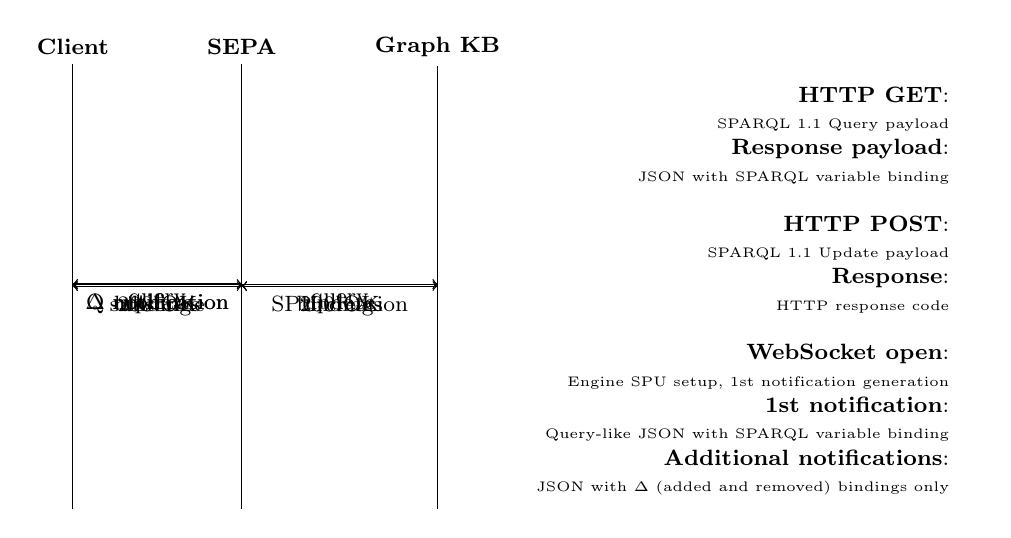
\begin{tikzpicture}[remember picture, 
    font=\footnotesize]

%Place a `comment` node with all text inside a tabular  
 \node(comments) {\begin{tabular}{r@{ }l}
        \subnode{A}{\textbf{HTTP GET}}:& \\
        \tiny{SPARQL 1.1 Query payload}\\
       \subnode{B}{\textbf{Response payload}}:& \\
       \tiny{JSON with SPARQL variable binding}\\[3mm]
       \subnode{C}{\textbf{HTTP POST}}:& \\
        \tiny{SPARQL 1.1 Update payload}\\
        \subnode{D}{\textbf{Response}}:& \\
       \tiny{HTTP response code}\\[3mm]
        \subnode{E}{\textbf{WebSocket open}}:& \\
       \tiny{Engine SPU setup, 1st notification generation}\\
        \subnode{F}{\textbf{1st notification}}:& \\
       \tiny{Query-like JSON with SPARQL variable binding}\\
        \subnode{G}{\textbf{Additional notifications}}:& \\
       \tiny{JSON with $\Delta$ (added and removed) bindings only}\\
       \end{tabular}};

% Place `server` and `client` nodes
\node[above left=1mm and 0mm of comments] (graphkb) {\textbf{Graph KB}}; 
\node[left=10mm of graphkb] (sepa) {\textbf{SEPA}}; 
\node[left=10mm of sepa] (client) {\textbf{Client}}; 

%Draw vertical lines
\draw (client) -- (client|-comments.south);
\draw (sepa) -- (sepa|-comments.south);
\draw (graphkb) -- (graphkb|-comments.south);

%Draw message interchanges
\draw[->, visible on=<1->] (A-|client)--node[below]{query} (A-|sepa) ;
\draw[->, visible on=<1->] (A-|sepa)--node[below]{query} (A-|graphkb) ;
\draw[->, visible on=<1->] (B-|graphkb)-- node[below]{bindings} (B-|sepa) ;
\draw[->, visible on=<1->] (B-|sepa)-- node[below]{bindings} (B-|client) ;

\draw[->, visible on=<2->] (C-|client)--node[below]{update} (C-|sepa) ;
\draw[->, visible on=<2->] (C-|sepa)--node[below]{update} (C-|graphkb) ;
\draw[->, visible on=<2->] (D-|graphkb)-- node[below]{200 OK} (D-|sepa) ;
\draw[->, visible on=<2->] (D-|sepa)-- node[below]{200 OK} (D-|client) ;

\draw[->, visible on=<3->] (E-|client)--node[below]{subscribe} (E-|sepa) ;
\draw[<->, visible on=<3->] (E-|sepa)--node[below]{SPU creation} (E-|graphkb) ;
\draw[->, visible on=<3->] (F-|sepa)-- node[below]{Q notification} (F-|client) ;
\draw[->, visible on=<4->] (G-|sepa)-- node[below]{$\Delta$ notification} (G-|client) ;
\end{tikzpicture}
\end{frame}

\begin{frame}[allowframebreaks]{AudioCommons project}
\framesubtitle{SEPA usage example}
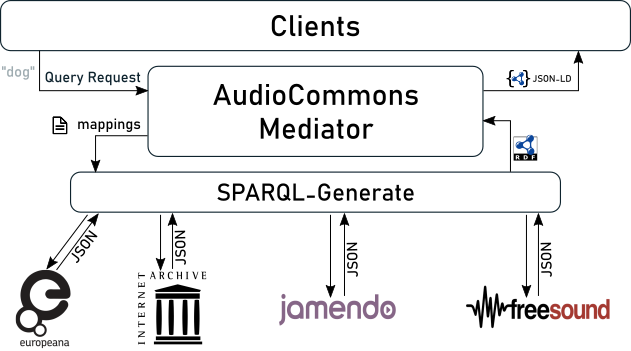
\includegraphics[width=\textwidth]{audiocommons_schema.png}
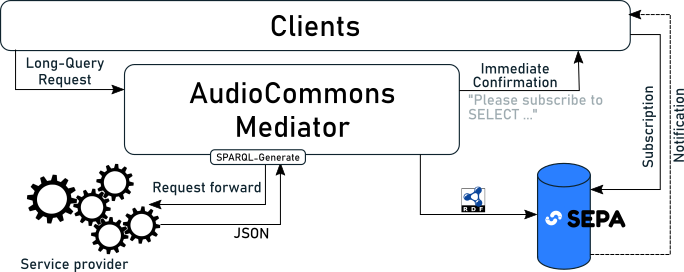
\includegraphics[width=\textwidth]{audiocommons_schema_sepa.png}
Ref. \cite{ceriani2018audio, xambo2018jam, lefranccois2017sparql}
\end{frame}

\subsection{W3C approach: Web of Things}
\begin{frame}[allowframebreaks]{Web of Things}
\framesubtitle{Prerequisite}
\begin{flushleft}
The Web of Things was introduced approximately in 2010 \cite{guinard2010resource}. The fragmentation of IoT was addressed considering that
\begin{itemize}
    \item the hardware available today is cheap and powerful;
    \item the World Wide Web stack, including HTTP protocol and JSON format for data exchange are broadly used;
    \item the RESTful design can be applied also to IoT systems and giving a broader meaning to the term `resource'
\end{itemize}

\framebreak
As discussed, the W3C provided its own definition of Thing, highlighting the fact that \textbf{they have URIs}.

\vspace{3mm}
The W3C WoT Working Group was created in this context to develop an interaction model and a common vocabulary to identify the Thing capabilities in the environment.

\vspace{3mm}
This Thesis work takes inspiration from the W3C drafts, and combines it with the aforementioned SEPA architecture \cite{antoniazzi2019building}.
\end{flushleft}
\end{frame}

\subsection{SWoT Ontology}
\begin{frame}{Comparison: W3C WoT vs SWoT ontology tools}
\small
\begin{tabular}{|p{.45\textwidth}|p{.45\textwidth}|}
\multicolumn{1}{c}{\textbf{W3C WoT}} & \multicolumn{1}{c}{\textbf{SWoT (this work)}} \\ \hline \hline
Devices have their \textbf{Thing Descriptions} (TD). They provide it as small web servers, in JSON-LD; & Devices post their TDs as a graph into SEPA; \\ \hline 
Clients still have to discover the devices by their own means, or discovery repos have to be implemented; & SEPA provides natively semantic discovery over the RDF graph of TDs; \\ \hline
Direct interaction after interpreting the TD; & SEPA-mediated interaction according to the  SWOT dynamic ontology \\ \hline
Reduced data model; & Extended data model and protocol; \\ \hline
No shared context, since TDs are separate universed; & SEPA may contain a shared context subgraph, depending on applications;\\ \hline \hline
\end{tabular}
\normalsize
\end{frame}

\begin{frame}{SWOT (static) Ontology}
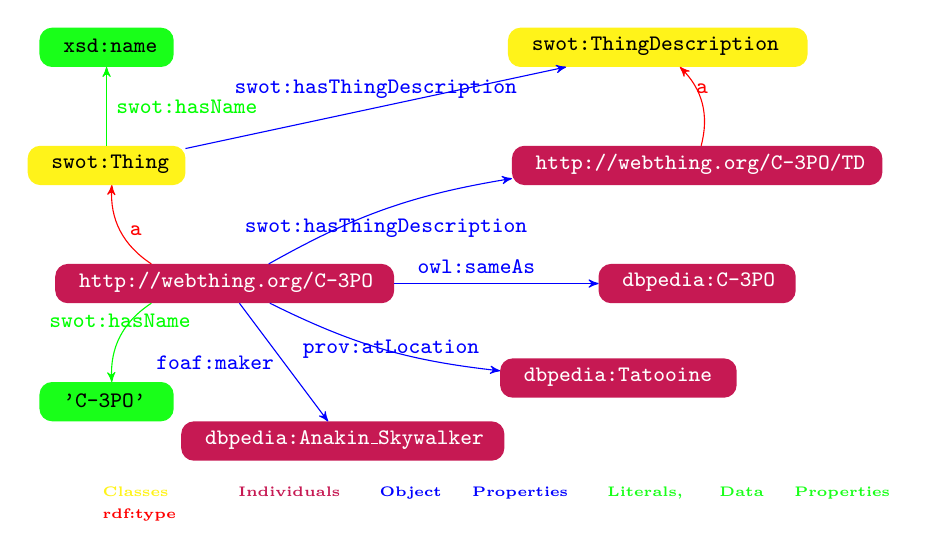
\begin{tikzpicture}[->,>=stealth']

\node[state,draw=yellow!90,fill=yellow!90,align=center, visible on=<1->] (THING) {
\begin{tabular}{l}
  \parbox{1.3cm}{\texttt{swot:Thing}}
   \end{tabular}
};
  
 % State: ACK with different content
 \node[state, right of=THING, node distance=7cm, yshift=1.5cm, anchor=center, draw=yellow!90,fill=yellow!90,align=center,visible on=<1->] (THINGDESCRIPTION) {%
    \begin{tabular}{l} 
        \parbox{3.1cm}{\texttt{swot:ThingDescription}}
    \end{tabular}
};


 % State: ACK with different content
 \node[state,  yshift=1.5cm, node distance=3cm, anchor=center, draw=green!90,fill=green!90,align=center, visible on=<1->] (THINGNAME) {%
    \begin{tabular}{l} 
        \parbox{1cm}{\texttt{xsd:name}}
    \end{tabular}
};

\onslide<2->{
   % State: ACK with different content
\node[state, yshift=-1.5cm, anchor=center, right of=THING, node distance=1.5cm, draw=purple!90,fill=purple!90,align=center,text=white,visible on=<2->] (C3PO) {%
    \begin{tabular}{l}
        \parbox{3.6cm}{\texttt{http://webthing.org/C-3PO}}
    \end{tabular}
};

 % State: ACK with different content
 \node[state,  yshift=-3cm, node distance=3cm, anchor=center, draw=green!90,fill=green!90,align=center,visible on=<2->] (C3PONAME) {%
    \begin{tabular}{l} 
        \parbox{1cm}{\texttt{'C-3PO'}}
    \end{tabular}
};
  
\node[state, right of=C3PO, yshift=-1.2cm, node distance=5cm, anchor=center, draw=purple!90,fill=purple!90,align=center,text=white,visible on=<2->] (TATOOINE) {%
    \begin{tabular}{l} 
        \parbox{2.3cm}{\texttt{dbpedia:Tatooine}}
    \end{tabular}
};

\node[state, anchor=center, 
right of=C3PO, 
draw=purple!90,fill=purple!90, yshift=1.5cm,
align=center,text=white, node distance=6cm,visible on=<2->] (C3POTD) {%
    \begin{tabular}{l}
        \parbox{4cm}{\texttt{http://webthing.org/C-3PO/TD}}
    \end{tabular}
};

 \node[state, right of=C3PO, node distance=6cm, anchor=center,draw=purple!90,fill=purple!90,text=white,align=center,visible on=<2->] (DBPEDIAC3PO) {%
    \begin{tabular}{l} 
        \parbox{1.8cm}{\texttt{dbpedia:C-3PO}}
    \end{tabular}
};

\node[state,yshift=-2cm,draw=purple!90,right of=C3PO, node distance=1.5cm, fill=purple!90,text=white,align=center,visible on=<2->] (ANAKIN) {
\begin{tabular}{l}
  \parbox{3.4cm}{\texttt{dbpedia:Anakin\_Skywalker}}
   \end{tabular}
};
}

\node[state,draw=none,right of=THING, node distance=5cm, yshift=-4.3cm,align=center,visible on=<1->] (LEGEND) {
\begin{tabular}{l}
  \parbox{10cm}{
  \textbf{\tiny{\textcolor{yellow!90}{Classes} \hspace{.5cm}\textcolor{purple!90}{Individuals}\hspace{.5cm}\textcolor{blue}{Object Properties}\hspace{.5cm}\textcolor{green!90}{Literals, Data Properties}}\hspace{.5cm}\textcolor{red}{rdf:type}}}
  \end{tabular}
};

\path 
(THING)     edge[draw=blue,visible on=<1->]  node[anchor=south,above]{\textcolor{blue}{\texttt{swot:hasThingDescription}}}   (THINGDESCRIPTION)
(THING)     edge[draw=green,visible on=<1->]  node[anchor=west]{\textcolor{green}{\texttt{swot:hasName}}}   (THINGNAME)
(C3PO)   edge[draw=red,bend left=30,visible on=<2->] node[anchor=west]{\textcolor{red}{\texttt{a}}}                      (THING)  
(C3POTD)   edge[draw=red, bend right=30,visible on=<2->] node[anchor=south, above]{\textcolor{red}{\texttt{a}}}  (THINGDESCRIPTION)  
(C3PO)   edge[draw=blue,bend left=10,visible on=<2->] node[anchor=north]{\textcolor{blue}{\texttt{swot:hasThingDescription}}}  (C3POTD)
(C3PO)     edge[draw=green, bend right=30,visible on=<2->] node[anchor=north west, above]{\textcolor{green}{\texttt{swot:hasName}}} (C3PONAME)
(C3PO)   edge[draw=blue, bend right=10,visible on=<2->] node[text width=2cm]{\textcolor{blue}{\texttt{prov:atLocation}}}                                (TATOOINE)
(C3PO)   edge[draw=blue,visible on=<2->] node[anchor=east]{\textcolor{blue}{\texttt{foaf:maker}}}                                (ANAKIN)
(C3PO)   edge[draw=blue, anchor=south,visible on=<2->] node[text width=2cm]{\textcolor{blue}{\texttt{owl:sameAs}}}                                (DBPEDIAC3PO)
;   

\end{tikzpicture}
\end{frame}
\begin{frame}{SWOT (static) Ontology}
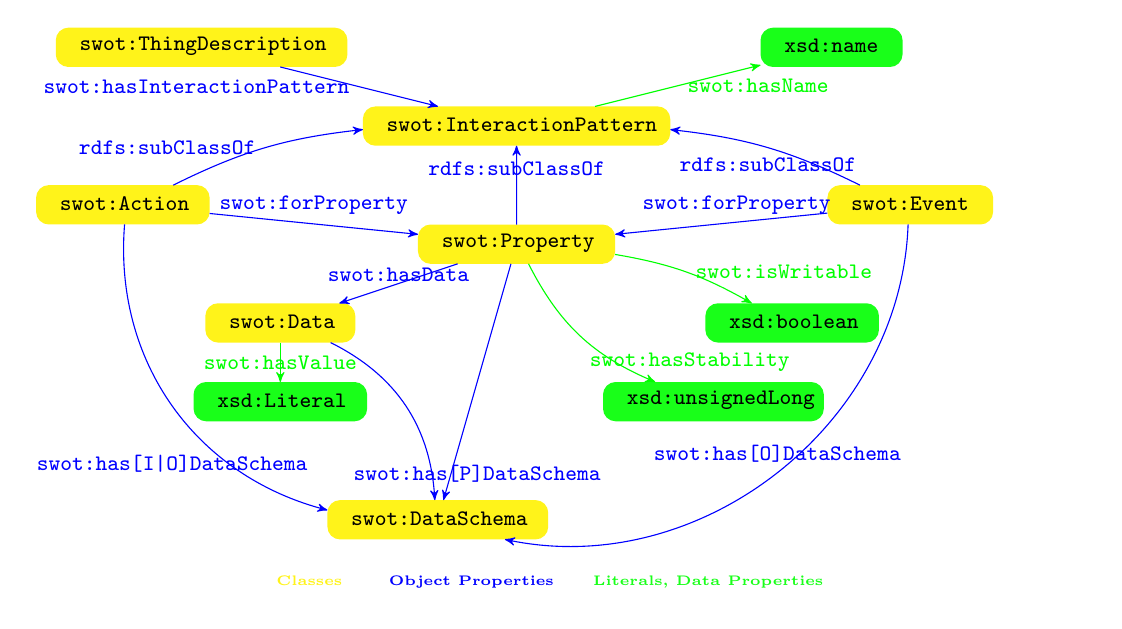
\begin{tikzpicture}[->,>=stealth']
  
 % State: ACK with different content
 \node[state, anchor=center, draw=yellow!90,fill=yellow!90,align=center,visible on=<1->] (THINGDESCRIPTION) {%
    \begin{tabular}{l} 
        \parbox{3cm}{\texttt{swot:ThingDescription}}
    \end{tabular}
};

 % State: ACK with different content
 \node[state,  yshift=-1cm, node distance=4cm, anchor=center, right of=THINGDESCRIPTION, draw=yellow!90,fill=yellow!90,align=center,visible on=<1->] (INTERACTIONPATTERN) {%
    \begin{tabular}{l} 
        \parbox{3.2cm}{\texttt{swot:InteractionPattern}}
    \end{tabular}
};
  
 % State: ACK with different content
 \node[state,  yshift=-2cm, node distance=-1cm, anchor=center, right of=THINGDESCRIPTION, draw=yellow!90,fill=yellow!90,align=center,visible on=<2->] (ACTION) {%
    \begin{tabular}{l} 
        \parbox{1.5cm}{\texttt{swot:Action}}
    \end{tabular}
};

   % State: ACK with different content
\node[state, yshift=-.5cm, anchor=center, right of=ACTION, node distance=5cm, draw=yellow!90,fill=yellow!90,align=center,visible on=<2->] (PROPERTY) {%
    \begin{tabular}{l}
        \parbox{1.8cm}{\texttt{swot:Property}}
    \end{tabular}
};
  
\node[state, right of=ACTION, node distance=10cm, anchor=center, draw=yellow!90,fill=yellow!90,align=center,visible on=<2->] (EVENT) {%
    \begin{tabular}{l} 
        \parbox{1.4cm}{\texttt{swot:Event}}
    \end{tabular}
};

\node[state, anchor=center, 
right of=ACTION, 
draw=yellow!90,fill=yellow!90, yshift=-1.5cm,
align=center, node distance=2cm,visible on=<3->] (DATA) {%
    \begin{tabular}{l}
        \parbox{1.2cm}{\texttt{swot:Data}}
    \end{tabular}
};

 \node[state, right of=ACTION, node distance=4cm, anchor=center,draw=yellow!90,fill=yellow!90,align=center, yshift=-4cm,visible on=<3->] (DATASCHEMA) {%
    \begin{tabular}{l} 
        \parbox{2.1cm}{\texttt{swot:DataSchema}}
    \end{tabular}
};

\node[state,draw=green!90,right of=DATA, node distance=6.5cm, fill=green!90,align=center,visible on=<3->] (BOOLEAN) {
\begin{tabular}{l}
  \parbox{1.5cm}{\texttt{xsd:boolean}}
   \end{tabular}
};

\node[state,draw=green!90,right of=DATA, node distance=5.5cm, fill=green!90,align=center,yshift=-1cm,visible on=<3->] (STABILITY) {
\begin{tabular}{l}
  \parbox{2.1cm}{\texttt{xsd:unsignedLong}}
   \end{tabular}
};

\node[state,yshift=-2.5cm,draw=green!90,right of=ACTION, node distance=2cm, fill=green!90,align=center,visible on=<3->] (LITERAL) {
\begin{tabular}{l}
  \parbox{1.5cm}{\texttt{xsd:Literal}}
   \end{tabular}
};

\node[state,draw=green!90,right of=THINGDESCRIPTION, node distance=8cm, fill=green!90,align=center,visible on=<1->] (NAME) {
\begin{tabular}{l}
  \parbox{1.1cm}{\texttt{xsd:name}}
   \end{tabular}
};



\node[state,draw=none,right of=DATASCHEMA, node distance=3cm, yshift=-.8cm,align=center] (LEGEND) {
\begin{tabular}{l}
  \parbox{10cm}{
  \textbf{\tiny{\textcolor{yellow!90}{Classes} \hspace{.5cm}\textcolor{blue}{Object Properties}\hspace{.5cm}\textcolor{green!90}{Literals, Data Properties}}}}
  \end{tabular}
};
 
\path (THINGDESCRIPTION)     edge[draw=blue,visible on=<1->]  node[anchor=east]{\textcolor{blue}{\texttt{swot:hasInteractionPattern}}}   (INTERACTIONPATTERN)
(INTERACTIONPATTERN)     edge[draw=green,visible on=<1->]  node[anchor=west]{\textcolor{green}{\texttt{swot:hasName}}}   (NAME)
(ACTION)   edge[draw=blue,bend left=10,visible on=<2->] node[anchor=east]{\textcolor{blue}{\texttt{rdfs:subClassOf}}}                      (INTERACTIONPATTERN)  
(PROPERTY)   edge[draw=blue,visible on=<2->] node[anchor=south, above]{\textcolor{blue}{\texttt{rdfs:subClassOf}}}  (INTERACTIONPATTERN)  
(EVENT)   edge[draw=blue,bend right=10,visible on=<2->] node[anchor=north]{\textcolor{blue}{\texttt{rdfs:subClassOf}}}  (INTERACTIONPATTERN)
(ACTION)     edge[draw=blue,visible on=<2->] node[anchor=north west, above]{\textcolor{blue}{\texttt{swot:forProperty}}} (PROPERTY)
(EVENT)   edge[draw=blue,visible on=<2->] node[text width=2cm,anchor=south]{\textcolor{blue}{\texttt{swot:forProperty}}}                                (PROPERTY)
(PROPERTY)   edge[draw=green, bend left=10,visible on=<3->] node[anchor=west]{\textcolor{green}{\texttt{swot:isWritable}}}                                (BOOLEAN)
(PROPERTY)   edge[draw=green, anchor=north west, bend right=20,visible on=<3->] node[text width=2cm,yshift=-.1cm]{\textcolor{green}{\texttt{swot:hasStability}}}                                (STABILITY)
(PROPERTY)   edge[draw=blue,visible on=<3->] node[anchor=north, above,yshift=-1.4cm]{\textcolor{blue}{\texttt{swot:has[P]DataSchema}}}  (DATASCHEMA)
(PROPERTY)   edge[draw=blue,visible on=<3->] node[anchor=south,yshift=-.1cm]{\textcolor{blue}{\texttt{swot:hasData}}}  (DATA)
(DATA)   edge[draw=green,visible on=<3->] node[]{\textcolor{green}{\texttt{swot:hasValue}}}  (LITERAL)
(DATA)   edge[draw=blue, bend left=30,visible on=<3->] node[]{}  (DATASCHEMA)
(EVENT)   edge[draw=blue, bend left=50,visible on=<3->] node[anchor=north, above]{\textcolor{blue}{\texttt{swot:has[O]DataSchema}}}  (DATASCHEMA)
(ACTION)   edge[draw=blue, bend right=40,visible on=<3->] node[anchor=north,yshift=-.5cm]{\textcolor{blue}{\texttt{swot:has[I|O]DataSchema}}}  (DATASCHEMA)
;   

\end{tikzpicture}
\end{frame}
\begin{frame}{SWOT (static) Ontology}
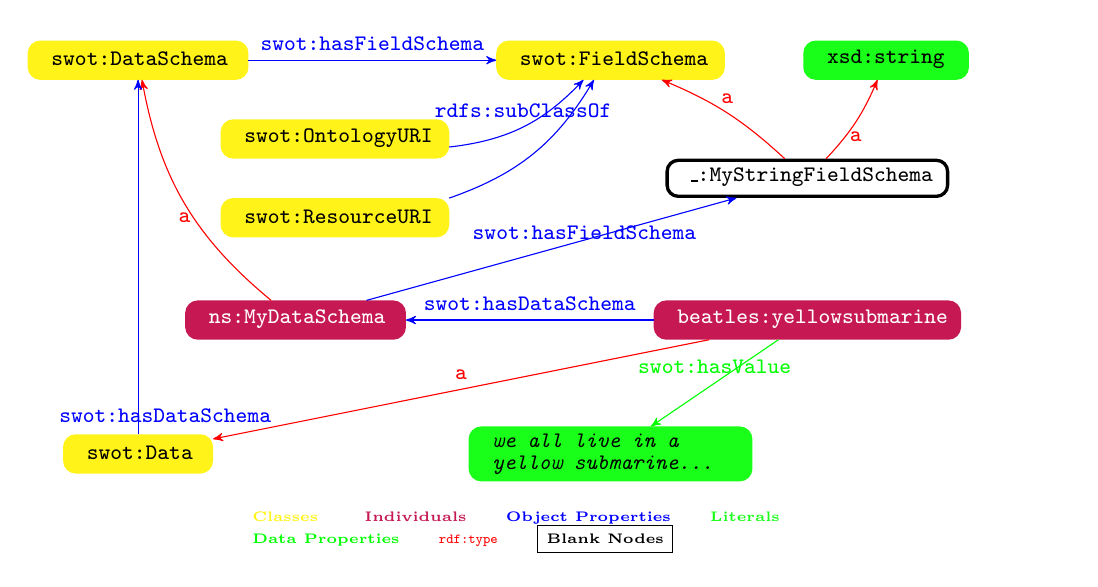
\begin{tikzpicture}[->,>=stealth']
  
 % State: ACK with different content
 \node[state, anchor=center, draw=yellow!90,fill=yellow!90,align=center,visible on=<1->] (DATASCHEMA) {%
    \begin{tabular}{l} 
        \parbox{2.1cm}{\texttt{swot:DataSchema}}
    \end{tabular}
};

 \node[state, anchor=center, yshift=-5cm, draw=yellow!90,fill=yellow!90,align=center,visible on=<1->] (DATA) {%
    \begin{tabular}{l} 
        \parbox{1.2cm}{\texttt{swot:Data}}
    \end{tabular}
};

 \node[state, anchor=center, right of=DATA, node distance=6cm, draw=green!90,fill=green!90,align=center,visible on=<2->] (SUBMARINE) {%
    \begin{tabular}{l} 
        \parbox{2.9cm}{\texttt{\textit{we all live in a yellow submarine...}}}
    \end{tabular}
};

 \node[state, anchor=center, right of=DATASCHEMA, draw=yellow!90,fill=yellow!90,align=center,node distance=6cm,visible on=<1->] (FIELDSCHEMA) {%
    \begin{tabular}{l} 
        \parbox{2.2cm}{\texttt{swot:FieldSchema}}
    \end{tabular}
};

 \node[state, anchor=center, right of=FIELDSCHEMA, draw=green!90,fill=green!90,align=center,node distance=3.5cm,visible on=<2->] (STRING) {%
    \begin{tabular}{l} 
        \parbox{1.4cm}{\texttt{xsd:string}}
    \end{tabular}
};

 \node[state, anchor=center, right of=DATASCHEMA, draw=yellow!90,fill=yellow!90,align=center,node distance=2.5cm,yshift=-1cm,visible on=<1->] (ONTOLOGYURI) {%
    \begin{tabular}{l} 
        \parbox{2.2cm}{\texttt{swot:OntologyURI}}
    \end{tabular}
};

 \node[state, anchor=center, right of=DATASCHEMA, draw=yellow!90,fill=yellow!90,align=center,node distance=2.5cm,yshift=-2cm,visible on=<1->] (RESOURCEURI) {%
    \begin{tabular}{l} 
        \parbox{2.2cm}{\texttt{swot:ResourceURI}}
    \end{tabular}
};

\node[state,right of=ONTOLOGYURI, node distance=6cm, yshift=-.5cm, align=center,visible on=<2->] (MSFS) {
\begin{tabular}{l}
  \parbox{2.9cm}{\texttt{\_:MyStringFieldSchema}}
   \end{tabular}
};

\node[state, right of=DATASCHEMA, yshift=-3.3cm, node distance=2cm, anchor=center, draw=purple!90,fill=purple!90,align=center,text=white,visible on=<2->] (MYDS) {%
    \begin{tabular}{l} 
        \parbox{2.1cm}{\texttt{ns:MyDataSchema}}
    \end{tabular}
};

\node[state, right of=MYDS, node distance=6.5cm, anchor=center, draw=purple!90,fill=purple!90,align=center,text=white,visible on=<2->] (BEATLES) {%
    \begin{tabular}{l} 
        \parbox{3.2cm}{\texttt{beatles:yellowsubmarine}}
    \end{tabular}
};

\node[state,draw=none,right of=DATA,node distance=6.5cm, yshift=-1cm,align=center] (LEGEND) {
\begin{tabular}{l}
  \parbox{10cm}{
  \textbf{\tiny{\textcolor{yellow!90}{Classes} \hspace{.5cm}\textcolor{purple!90}{Individuals}\hspace{.5cm}\textcolor{blue}{Object Properties}\hspace{.5cm}\textcolor{green!90}{Literals}\\\textcolor{green}{ Data Properties}\hspace{.5cm}\textcolor{red}{\texttt{rdf:type}}\hspace{.5cm}\framebox{Blank Nodes}}}}
  \end{tabular}
};
 
 
\path (DATASCHEMA)     edge[draw=blue,visible on=<1->]  node[anchor=south]{\textcolor{blue}{\texttt{swot:hasFieldSchema}}}   (FIELDSCHEMA)
(ONTOLOGYURI)     edge[draw=blue, bend right=20,visible on=<1->]  node[anchor=south]{\textcolor{blue}{\texttt{rdfs:subClassOf}}}   (FIELDSCHEMA)
(RESOURCEURI)   edge[draw=blue,bend right=20,visible on=<1->] node[]{}                (FIELDSCHEMA)  
(MSFS)   edge[draw=red,bend right=10,visible on=<2->] node[anchor=south, above]{\textcolor{red}{\texttt{a}}}  (FIELDSCHEMA)  
(MSFS)   edge[draw=red,bend right=10,visible on=<2->] node[anchor=north]{\textcolor{red}{\texttt{a}}}  (STRING)
(MYDS)     edge[draw=red, bend left=20,visible on=<2->] node[anchor=north]{\textcolor{red}{\texttt{a}}} (DATASCHEMA)
(MYDS)   edge[draw=blue,visible on=<2->] node[text width=2cm,anchor=south]{\textcolor{blue}{\texttt{swot:hasFieldSchema}}}     (MSFS)
(BEATLES)   edge[draw=blue,visible on=<2->] node[anchor=south]{\textcolor{blue}{\texttt{swot:hasDataSchema}}}       (MYDS)
(DATA)   edge[draw=blue, anchor=north,visible on=<1->] node[text width=2cm,yshift=-1.8cm]{\textcolor{blue}{\texttt{swot:hasDataSchema}}}                                (DATASCHEMA)
(BEATLES)   edge[draw=green,visible on=<2->] node[anchor=north, above]{\textcolor{green}{\texttt{swot:hasValue}}}  (SUBMARINE)
(BEATLES)   edge[draw=red,visible on=<2->] node[anchor=south]{\textcolor{red}{\texttt{a}}}  (DATA)
;   

\end{tikzpicture}
\end{frame}

\begin{frame}{SWOT (dynamic) Ontology}
\framesubtitle{Triggering an Action Request}
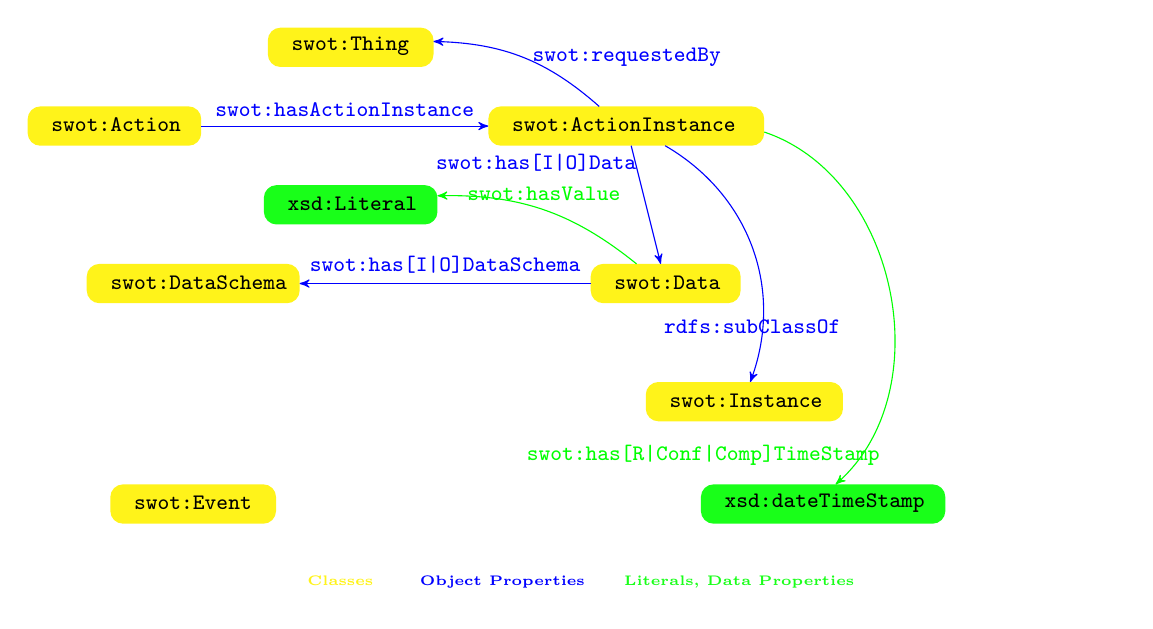
\begin{tikzpicture}[->,>=stealth']
  
 % State: ACK with different content
 \node[state, anchor=center, draw=yellow!90,fill=yellow!90,align=center,visible on=<1->] (ACTION) {%
    \begin{tabular}{l} 
        \parbox{1.5cm}{\texttt{swot:Action}}
    \end{tabular}
};

 \node[state, anchor=center, right of=ACTION, node distance=6.5cm, draw=yellow!90,fill=yellow!90,align=center,visible on=<2->] (ACTIONINSTANCE) {%
    \begin{tabular}{l} 
        \parbox{2.8cm}{\texttt{swot:ActionInstance}}
    \end{tabular}
};

 \node[state, anchor=center, right of=ACTION, node distance=3cm, yshift=1cm, draw=yellow!90,fill=yellow!90,align=center,visible on=<2->] (THING) {%
    \begin{tabular}{l} 
        \parbox{1.4cm}{\texttt{swot:Thing}}
    \end{tabular}
};

 \node[state, anchor=center, right of=ACTION, node distance=1cm, yshift=-2cm, draw=yellow!90,fill=yellow!90,align=center,visible on=<2->] (DATASCHEMA) {%
    \begin{tabular}{l} 
        \parbox{2cm}{\texttt{swot:DataSchema}}
    \end{tabular}
};
 
 \node[state, anchor=center, right of=DATASCHEMA, node distance=6cm,  draw=yellow!90,fill=yellow!90,align=center,visible on=<2->] (DATA) {%
    \begin{tabular}{l} 
        \parbox{1.2cm}{\texttt{swot:Data}}
    \end{tabular}
};

 \node[state, anchor=center, right of=DATASCHEMA, node distance=2cm, yshift=1cm, draw=green!90,fill=green!90,align=center,visible on=<2->] (LITERAL) {%
    \begin{tabular}{l} 
        \parbox{1.5cm}{\texttt{xsd:Literal}}
    \end{tabular}
};

% \node[state, anchor=center, right of=ACTION, node distance=1cm, yshift=-3.5cm, draw=yellow!90,fill=yellow!90,align=center,draw=none] (EVENTINSTANCE) {%
%    \begin{tabular}{l} 
%        \parbox{2.5cm}{\texttt{swot:EventInstance}}
%    \end{tabular}
%};
 
 \node[state, anchor=center, right of=ACTION, node distance=8cm, yshift=-3.5cm, draw=yellow!90,fill=yellow!90,align=center,visible on=<2->] (INSTANCE) {%
    \begin{tabular}{l} 
        \parbox{1.8cm}{\texttt{swot:Instance}}
    \end{tabular}
};

 \node[state, anchor=center, right of=ACTION, node distance=1cm, yshift=-4.8cm, draw=yellow!90,fill=yellow!90,align=center,visible on=<1->] (EVENT) {%
    \begin{tabular}{l} 
        \parbox{1.4cm}{\texttt{swot:Event}}
    \end{tabular}
};

 \node[state, anchor=center, right of=ACTION, node distance=9cm,yshift=-4.8cm, draw=green!90,fill=green!90,align=center,visible on=<2->] (DTS) {%
    \begin{tabular}{l} 
        \parbox{2.4cm}{\texttt{xsd:dateTimeStamp}}
    \end{tabular}
};

\node[state,draw=none,right of=ACTION, node distance=7.5cm, yshift=-5.8cm,align=center] (LEGEND) {
\begin{tabular}{l}
  \parbox{10cm}{
  \textbf{\tiny{\textcolor{yellow!90}{Classes} \hspace{.5cm}\textcolor{blue}{Object Properties}\hspace{.5cm}\textcolor{green!90}{Literals, Data Properties}}}}
  \end{tabular}
};
 
\path (ACTIONINSTANCE)     edge[draw=blue, bend right=20,visible on=<2->]  node[anchor=west]{\textcolor{blue}{\texttt{swot:requestedBy}}}   (THING)
(ACTION)     edge[draw=blue,visible on=<2->]  node[anchor=south]{\textcolor{blue}{\texttt{swot:hasActionInstance}}}   (ACTIONINSTANCE)
(ACTIONINSTANCE)   edge[draw=blue,bend left=40,visible on=<2->] node[yshift=-1cm]{\textcolor{blue}{\texttt{rdfs:subClassOf}}}                (INSTANCE)  
(ACTIONINSTANCE)   edge[draw=green,bend left=60,visible on=<2->] node[anchor=east,yshift=-2.1cm]{\textcolor{green}{\texttt{swot:has[R|Conf|Comp]TimeStamp}}}  (DTS)  
%(EVENTINSTANCE)   edge[draw=green,bend right=10] node[anchor=north]{\textcolor{green}{\texttt{swot:occurredAt}}}  (DTS)
%(EVENTINSTANCE)     edge[draw=blue] node[anchor=south]{\textcolor{blue}{\texttt{rdfs:subClassOf}}} (INSTANCE)
%(EVENTINSTANCE)   edge[draw=blue] node[text width=2cm,anchor=south]{\textcolor{blue}{\texttt{swot:has[O]Data}}}     (DATA)
(DATA)   edge[draw=blue,visible on=<2->] node[anchor=south]{\textcolor{blue}{\texttt{swot:has[I|O]DataSchema}}}       (DATASCHEMA)
%(EVENT)   edge[draw=blue] node[text width=2cm,yshift=.4]{\textcolor{blue}{\texttt{swot:hasEventInstance}}}   (EVENTINSTANCE)
(DATA)   edge[draw=green, bend right=20,visible on=<2->] node[anchor=west, above]{\textcolor{green}{\texttt{swot:hasValue}}}  (LITERAL)
(ACTIONINSTANCE)   edge[draw=blue,visible on=<2->] node[anchor=south east, yshift=.3cm]{\textcolor{blue}{\texttt{swot:has[I|O]Data}}}  (DATA)
;   

\end{tikzpicture}
\end{frame}
\begin{frame}{SWOT (dynamic) Ontology}
\framesubtitle{Triggering an Event Notification}
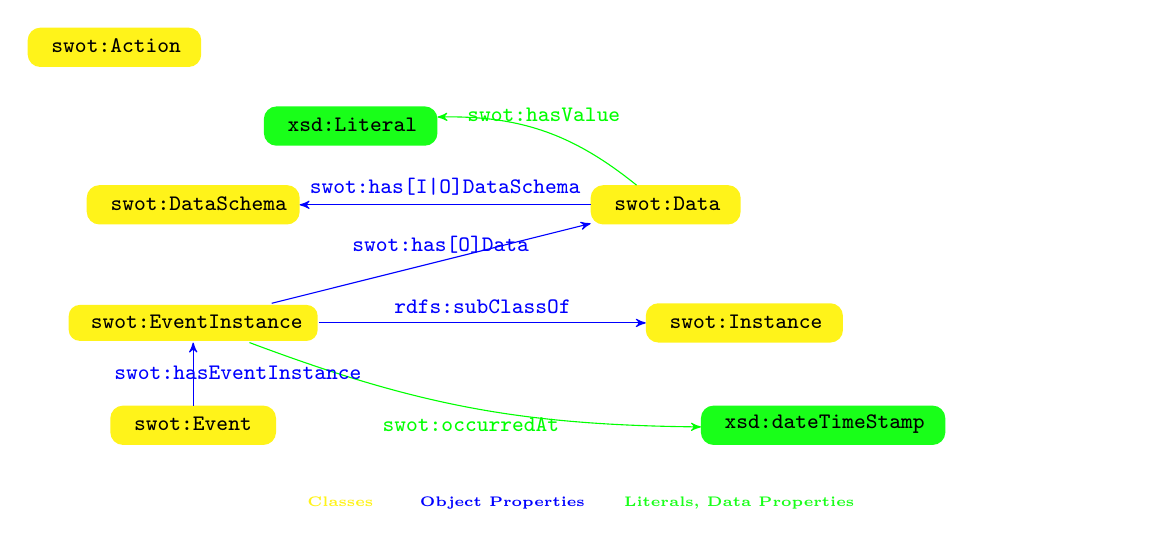
\begin{tikzpicture}[->,>=stealth']
  
  State: ACK with different content
 \node[state, anchor=center, draw=yellow!90,fill=yellow!90,align=center,visible on=<1->] (ACTION) {%
    \begin{tabular}{l} 
        \parbox{1.5cm}{\texttt{swot:Action}}
    \end{tabular}
};

 %\node[state, anchor=center, right of=ACTION, node distance=6.5cm, draw=yellow!90,fill=yellow!90,align=center,visible on=<2->] (ACTIONINSTANCE) {%
 %   \begin{tabular}{l} 
 %       \parbox{2.8cm}{\texttt{swot:ActionInstance}}
 %   \end{tabular}
%};

% \node[state, anchor=center, right of=ACTION, node distance=3cm, yshift=1cm, draw=yellow!90,fill=yellow!90,align=center,visible on=<2->] (THING) {%
%    \begin{tabular}{l} 
%        \parbox{1.4cm}{\texttt{swot:Thing}}
%    \end{tabular}
%};

 \node[state, anchor=center, right of=ACTION, node distance=1cm, yshift=-2cm, draw=yellow!90,fill=yellow!90,align=center,visible on=<2->] (DATASCHEMA) {%
    \begin{tabular}{l} 
        \parbox{2cm}{\texttt{swot:DataSchema}}
    \end{tabular}
};
 
 \node[state, anchor=center, right of=DATASCHEMA, node distance=6cm,  draw=yellow!90,fill=yellow!90,align=center,visible on=<2->] (DATA) {%
    \begin{tabular}{l} 
        \parbox{1.2cm}{\texttt{swot:Data}}
    \end{tabular}
};

 \node[state, anchor=center, right of=DATASCHEMA, node distance=2cm, yshift=1cm, draw=green!90,fill=green!90,align=center,visible on=<2->] (LITERAL) {%
    \begin{tabular}{l} 
        \parbox{1.5cm}{\texttt{xsd:Literal}}
    \end{tabular}
};

 \node[state, anchor=center, right of=ACTION, node distance=1cm, yshift=-3.5cm, draw=yellow!90,fill=yellow!90,align=center,draw=none,visible on=<2->] (EVENTINSTANCE) {%
   \begin{tabular}{l} 
        \parbox{2.5cm}{\texttt{swot:EventInstance}}
    \end{tabular}
};
 
 \node[state, anchor=center, right of=ACTION, node distance=8cm, yshift=-3.5cm, draw=yellow!90,fill=yellow!90,align=center,visible on=<2->] (INSTANCE) {%
    \begin{tabular}{l} 
        \parbox{1.8cm}{\texttt{swot:Instance}}
    \end{tabular}
};

 \node[state, anchor=center, right of=ACTION, node distance=1cm, yshift=-4.8cm, draw=yellow!90,fill=yellow!90,align=center,visible on=<1->] (EVENT) {%
    \begin{tabular}{l} 
        \parbox{1.4cm}{\texttt{swot:Event}}
    \end{tabular}
};

 \node[state, anchor=center, right of=ACTION, node distance=9cm,yshift=-4.8cm, draw=green!90,fill=green!90,align=center,visible on=<2->] (DTS) {%
    \begin{tabular}{l} 
        \parbox{2.4cm}{\texttt{xsd:dateTimeStamp}}
    \end{tabular}
};

\node[state,draw=none,right of=ACTION, node distance=7.5cm, yshift=-5.8cm,align=center] (LEGEND) {
\begin{tabular}{l}
  \parbox{10cm}{
  \textbf{\tiny{\textcolor{yellow!90}{Classes} \hspace{.5cm}\textcolor{blue}{Object Properties}\hspace{.5cm}\textcolor{green!90}{Literals, Data Properties}}}}
  \end{tabular}
};
 
\path 
%(ACTIONINSTANCE)     edge[draw=blue, bend right=20,visible on=<2->]  node[anchor=west]{\textcolor{blue}{\texttt{swot:requestedBy}}}   (THING)
%(ACTION)     edge[draw=blue,visible on=<2->]  node[anchor=south]{\textcolor{blue}{\texttt{swot:hasActionInstance}}}   (ACTIONINSTANCE)
%(ACTIONINSTANCE)   edge[draw=blue,bend left=40,visible on=<2->] node[yshift=-1cm]{\textcolor{blue}{\texttt{rdfs:subClassOf}}}                (INSTANCE)  
%(ACTIONINSTANCE)   edge[draw=green,bend left=60,visible on=<2->] node[anchor=east,yshift=-2.1cm]{\textcolor{green}{\texttt{swot:has[R|Conf|Comp]TimeStamp}}}  (DTS)  
(EVENTINSTANCE)   edge[draw=green,bend right=10,visible on=<2->] node[anchor=north]{\textcolor{green}{\texttt{swot:occurredAt}}}  (DTS)
(EVENTINSTANCE)     edge[draw=blue,visible on=<2->] node[anchor=south]{\textcolor{blue}{\texttt{rdfs:subClassOf}}} (INSTANCE)
(EVENTINSTANCE)   edge[draw=blue,visible on=<2->] node[text width=2cm,anchor=south]{\textcolor{blue}{\texttt{swot:has[O]Data}}}     (DATA)
(DATA)   edge[draw=blue,visible on=<2->] node[anchor=south]{\textcolor{blue}{\texttt{swot:has[I|O]DataSchema}}}       (DATASCHEMA)
(EVENT)   edge[draw=blue,visible on=<2->] node[text width=2cm,yshift=.4]{\textcolor{blue}{\texttt{swot:hasEventInstance}}}   (EVENTINSTANCE)
(DATA)   edge[draw=green, bend right=20,visible on=<2->] node[anchor=west, above]{\textcolor{green}{\texttt{swot:hasValue}}}  (LITERAL)
%(ACTIONINSTANCE)   edge[draw=blue,visible on=<2->] node[anchor=south east, yshift=.3cm]{\textcolor{blue}{\texttt{swot:has[I|O]Data}}}  (DATA)
;   

\end{tikzpicture}
\end{frame}
\begin{frame}
\includegraphics[width=\textwidth]{swot_screenshot.png}
\texttt{https://fr4ncidir.github.io/SemanticWoT/}
\end{frame}

\section{Programming the SWoT}
\subsection{Cocktail Framework}
\begin{frame}{Cocktail Framework}
A Python3 framework was developed to fully exploit the SWOT ontology presented, based on a SEPA engine:
\begin{enumerate}
    \item<1-> semantic TD definition and posting;
    \item<2-> event subscription and notification;
    \item<3-> action request and execution;
    \item<4-> full semantic discovery;
\end{enumerate}
All this by using SEPA's engine with SPARQL 1.1 Queries, Updates and Discoveries.
\end{frame}

\subsection{Typical Workflow}
\begin{frame}{SWoT Application Workflow}
\framesubtitle{Basic example with two devices}
\begin{tikzpicture}[
    node distance=2cm,
    every node/.style={fill=white, font=\fontsize{8pt}{8}\selectfont}, 
    align=center, 
    base/.style = {
        rectangle, rounded corners, draw=black,
        minimum width=1cm, minimum height=0.5cm,
        text centered, font=\fontsize{8pt}{8}\selectfont},
    ]
        

  % Specification of nodes (position, etc.)
\node (one)   [base, visible on=<1->]  {
\begin{tabular}{cc}
\multirow{2}{*}{\includegraphics[scale=.05]{rpi.png}} & R$\pi$ connects \\ & to \faWifi
\end{tabular}};

\node (two)     [base, right of=one, node distance=4cm, visible on=<2->] {
\begin{tabular}{cc}
\multirow{2}{*}{\includegraphics[scale=.05]{rpi.png}} & R$\pi$ updates its \\ & TD to SEPA
\end{tabular}};

\node (three) [base, right of=two, node distance=4cm, visible on=<3->]   {\begin{tabular}{cc}
\multirow{3}{*}{\includegraphics[scale=.05]{rpi.png}} & R$\pi$ subscribes for \\ & other Things it \\ & can contact
\end{tabular}};

\node (wait) [right of=three, node distance=0cm, yshift=-1cm, visible on=<3->]{wait...};

\node (four) [base, right of=two, node distance=3.4cm, yshift=-2.1cm, visible on=<4->]   {\begin{tabular}{cc}
\multirow{3}{*}{\includegraphics[scale=.035]{arduino.jpeg}} & appears and updates \\ & its TD to SEPA. It \\ & fulfils R$\pi$ requests
\end{tabular}};

\node (five) [base, right of=two, node distance=.7cm, yshift=-1cm, visible on=<5->]   {\begin{tabular}{cc}
\multirow{2}{*}{\includegraphics[scale=.05]{rpi.png}} & R$\pi$ is notified \\ & about Arduino
\end{tabular}};

\node (six) [base, right of=one, node distance=.5cm, yshift=-1.8cm, visible on=<6->]   {\begin{tabular}{cc}
\multirow{3}{*}{\includegraphics[scale=.05]{rpi.png}} & R$\pi$ checks the envi-
 \\ & ronment: is it necessary\\ & to trigger actuation?
\end{tabular}};

\node (seven) [base, right of=six, node distance=-1.5cm, yshift=-1.3cm, visible on=<7->]   {wait...};

\node (eight) [base, right of=two, node distance=-1cm, yshift=-3cm, visible on=<8->]   {\begin{tabular}{cc}
\multirow{2}{*}{\includegraphics[scale=.05]{rpi.png}} & R$\pi$ updates a new\\ & request for Arduino
\end{tabular}};

\node (nine) [base, right of=eight, node distance=4.4cm,yshift=-1cm, visible on=<9->]   {\begin{tabular}{cc}
\multirow{3}{*}{\includegraphics[scale=.05]{rpi.png}} & An output is expected. 
 \\ & R$\pi$ subscribes \\ & to Arduino output
\end{tabular}};

\node (ten) [base, right of=nine, node distance=0cm, yshift=-1.7cm, visible on=<10->]   {\begin{tabular}{cc}
\multirow{3}{*}{\includegraphics[scale=.035]{arduino.jpeg}} & Arduino is notified \\ & of a new \\ & actuation request
\end{tabular}};

\node (eleven) [base, left of=ten, node distance=4.5cm, visible on=<11->]   {\begin{tabular}{cc}
\multirow{3}{*}{\includegraphics[scale=.035]{arduino.jpeg}} & Arduino performs \\ & its tasks and\\ & Updates its output
\end{tabular}};

\node (twelve) [base, left of=eleven, node distance=0cm, yshift=1.4cm, visible on=<12->]   {\begin{tabular}{cc}
\multirow{2}{*}{\includegraphics[scale=.05]{rpi.png}} & R$\pi$ is notified \\ & about the output
\end{tabular}};
  
  % Specification of lines between nodes specified above
  % with aditional nodes for description 
  \draw[->, visible on=<2->] (one) -- (two);
  \draw[->, visible on=<3->]     (two) -- (three);
  \draw[->, visible on=<3->]  (three) -- (wait) -| (four);
  \draw[->, visible on=<5->]      (four) -| (five);
  \draw[->, visible on=<6->]     (five) -| (six);
  \draw[<->, visible on=<7->]      (six) |- node{no} (seven);
  \draw[->, visible on=<8->]      (six) -| node[anchor=west, yshift=-.4cm]{yes} (eight);
  \draw[->, visible on=<9->]    (eight) -| (nine);
  \draw[->, visible on=<10->]       (nine) -- (ten);
  \draw[->, visible on=<11->]    (ten) -- (eleven);
  \draw[->, visible on=<12->]      (eleven) -- (twelve);
  \draw[->, visible on=<13->]    (twelve) -| node{\texttt{while (1)}\\ loop restart} (seven);
  \end{tikzpicture}
\end{frame}

\section{Future Research...}
\begin{frame}{Future Research...}
\begin{itemize}
    \item<1-> From the Internet of Musical Things to the (Semantic) Web of Musical Things; \\ \textit{\footnotesize{In collaboration with Università di Trento}}
    \item<2-> enhance SPARQL-Generate; \\
    \textit{\footnotesize{PostDoc at \'{E}cole des Mines de St-\'{E}tienne}}
    \item<3-> Apply the workflow previously presented to create Industry 4.0 environments;
    \textit{\footnotesize{\'{E}cole des Mines de St-\'{E}tienne}: IT'M Factory}
    \item<4-> Study additional coordination mechanisms on these environments;
    \textit{\footnotesize{\'{E}cole des Mines de St-\'{E}tienne}: Plateforme Territoire}
\end{itemize}
\end{frame}


\begin{frame}%[allowframebreaks]
\begin{tiny}
\frametitle{References}
\bibliographystyle{ieeetr}
\setbeamertemplate{bibliography item}{\insertbiblabel}
\bibliography{biblio.bib}
\end{tiny}
\end{frame}

\begin{frame}
\begin{tikzpicture}
\draw (0, 0) node[inner sep=0] {\includegraphics[width=\textwidth]{questions.jpg}};
\draw (1, -2) node {\textbf{\textit{\Huge{\textcolor{white}{Questions?}}}}};
\end{tikzpicture}
\end{frame}

\end{document}
